
% ------------------------------------------------------------
% ------------------------------------------------------------

\section[Geographical Plots]{Geographical Plots}
%%%%%%%%%%%%%%%%%%%%%%%%%%%%%%%%%%%%%
\subsection{Plots using Maps}
%%%%%%%%%%%%%%%%%%%%%%%%%%%%%%%%%%%%%

\begin{frame}[fragile, allowframebreaks]
\frametitle{Geographic Maps (v0.1)}

To overlay a map to a plot containing latitude and longitude, load the package \ttfamily maps: \normalfont 

\begin{lstlisting}[ basicstyle=\footnotesize]
library(maps)
plot(
 x = df_clean$Longitude, 
 y = df_clean$Latitude,
 xlab = "Longitude",
 ylab = "Latitude",
 pch = 16,
 col = rgb(176/256, 196/256, 222/256, alpha=0.5)
)
map("state", "california", add=TRUE)
\end{lstlisting}

\newpage
	\begin{center}
		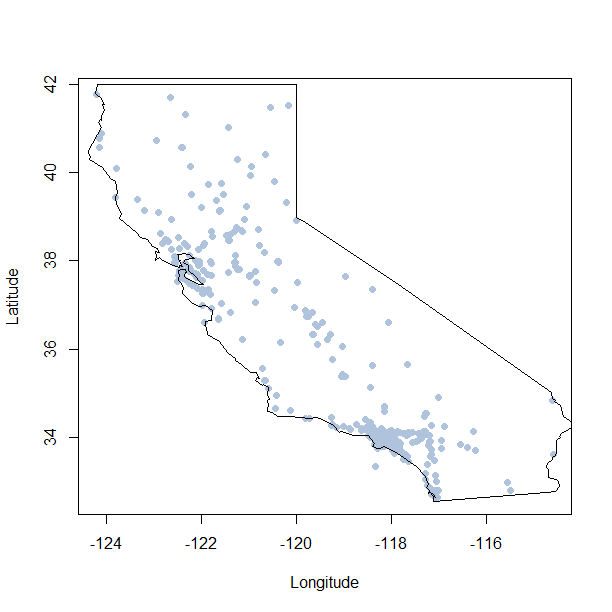
\includegraphics[scale=0.25]{images/geoplot_v0.png}
	\end{center}
What are some limitations of the plot?
\end{frame}

%___________
\begin{frame}[fragile, allowframebreaks]
\frametitle{Geographic Maps (v0.2)}

To include information on volume of procedure, use \ttfamily cex\normalfont argument of the \ttfamily plot() \normalfont function:

\begin{lstlisting}[ basicstyle=\footnotesize]
### Step 1: Aggregate data to be at hospital level:
df_hosp <- data_clean %>%
  group_by( Latitude, Longitude ) %>%
  summarise( Total.for.Hospital = sum(Volume, na.rm=TRUE) )
	
### Step 2: Recode 'Volume' to have 2 categories only: high ( >100 cases ) and low ( <= 100 cases ):
df_hosp$volume_ind <- ifelse( 
 test = df_hosp$Total.for.Hospital > 100, 
 yes = 2, 
 no = 1 )
\end{lstlisting}

\newpage
\begin{lstlisting}
### Step 3: Plot
plot(
 x = df_hosp$Longitude, 
 y = df_hosp$Latitude, 
 pch = 19, 
 cex = df_hosp$volume_ind, 
 col = df_hosp$volume_ind, 
 xlab = "Longitude", 
 ylab = "Latitude",
 main="Indicator of overall volume between 2005-2014"
)
map("state", "california", add=TRUE)
\end{lstlisting}

\begin{lstlisting}
### Step 4: Add legend
legend("topright", 
 pch = 19, 
 pt.cex = 1:2,
 col = 1:2, 
 c("Vol <= 100", "Vol > 100") 
)
\end{lstlisting}

\newpage
       \begin{center}
		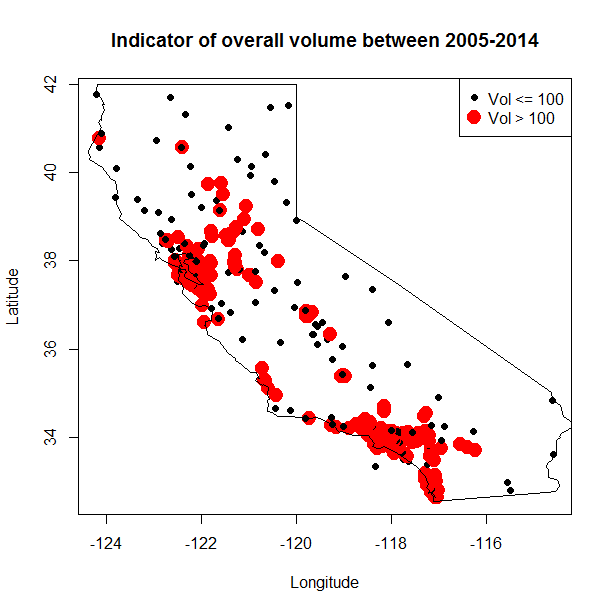
\includegraphics[scale=0.25]{images/geoplot_v1.png}
	\end{center}
What are some limitations of the plot? (Exercise.)
\end{frame}

%---
\begin{frame}[fragile, allowframebreaks]
\frametitle{Geographic Maps (v0.3)}

Another way to visualize geographical information is via shapefiles. Please download shapefiles for California for 2014 from \url{https://www.census.gov/geo/maps-data/data/cbf/cbf_tracts.html} and unzip the folder.

\begin{lstlisting}
### Step 1: Load in required packages
library(sp)
library(rgdal)
\end{lstlisting}

\newpage
\begin{lstlisting}
### Step 2: Read in shapefile and add latitude and longitude cordinates to it:
tracts = spTransform(
	readOGR(
		file.path("cb_2014_06_tract_500k"), 
		layer = "cb_2014_06_tract_500k"
		), 
	CRS("+proj=longlat +datum=WGS84")
	) 

### Step 3: Visualize
plot(tracts)
\end{lstlisting}

\newpage
       \begin{center}
		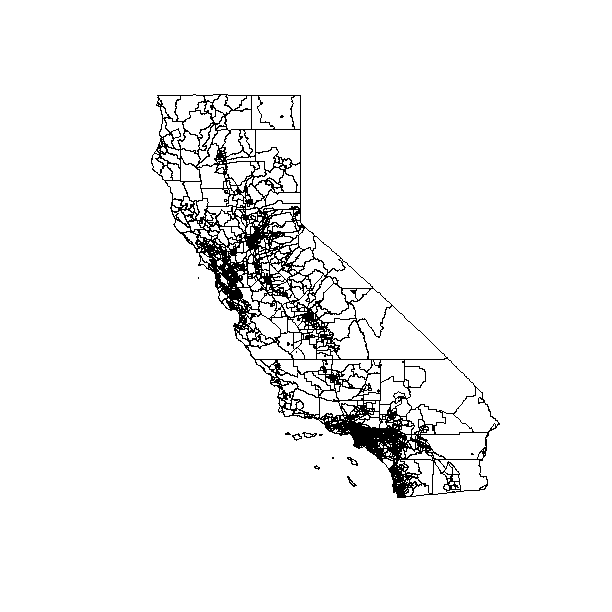
\includegraphics[scale=0.25]{images/shapefile_v0.png}
		\caption{Plot of the shapefile tracts.}
	\end{center}

\newpage
Now let's add the locations of hospitals to the map [12]:

\begin{lstlisting}
### Step 1: Load required packages
library("rgdal") 
library("maptools")
library("ggplot2")
library("plyr")

### Step 2: Preprocess data ahead of plotting
tracts@data$id = rownames(tracts@data)
tracts.points = fortify(tracts, region="id")
tracts.df = join(
 tracts.points, 
 tracts@data, 
 by="id"
 )
\end{lstlisting}

\newpage
\begin{lstlisting}
### Step 3: Visualize
ggplot() +
  geom_polygon(data = tracts.df,
               aes(x = long, y = lat, group = group),
               fill = grey(0.6), 
               color = grey(0.6), 
               alpha = 0.5
               ) + 
  geom_point(data = df_hosp,
             aes(x = Longitude, y = Latitude),
             color = "blue4", 
             alpha = 0.5, 
             shape = 3,
             size = 2 )
\end{lstlisting}

\newpage
       \begin{center}
		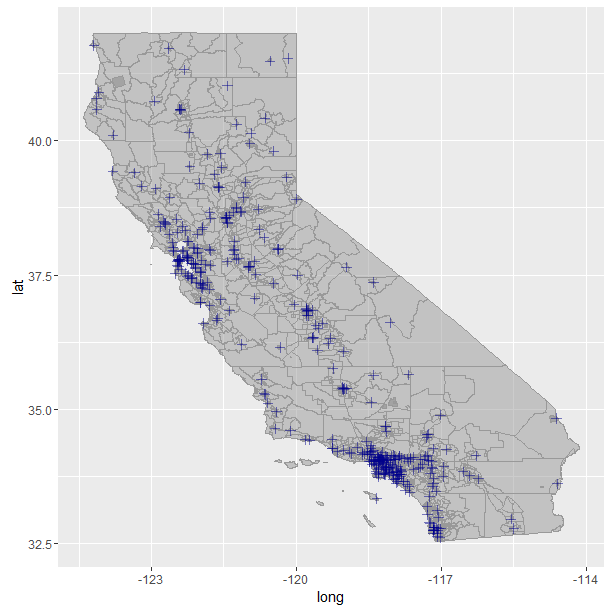
\includegraphics[scale=0.3]{images/shapefile_v1.png}
	\end{center}

\end{frame}

% %%%%%%%%%%%
% \begin{frame}[fragile]
% 	\begin{alertblock}{Bonus Feature of the \ttfamily maps \normalfont package:}
% 		To determine in which part of the world the observations are (based on latitude and longitude), use \ttfamily map.where(): \normalfont
% 			\begin{lstlisting}		
% 				in.what.country<-map.where(database="world", quakes$long, quakes$lat)
% 			\end{lstlisting}
% 		To determine which observations are in the ocean: \normalfont
% 			\begin{lstlisting}
% 				# Number of points in ocean after filtering:
% 				ind<-sum(is.na(in.what.country)); ind
% 				# Number of observations: 1000
% 				# Number in Ocean: 993
% 			\end{lstlisting}
% 	\end{alertblock}

% \end{frame}

% ------------------------------------------------------------
% ------------------------------------------------------------
\subsection{Exercise III}
\begin{frame}
	\frametitle{Exercise III}
	For the \ttfamily ozone \normalfont data set \footnote{\ttfamily http://www.ats.ucla.edu/stat/R/faq/ozone.csv\normalfont}, determine the region of the world that the observations correspond to and overlay the appropriate map.
\end{frame}
%ozone<-read.table("http://www.ats.ucla.edu/stat/R/faq/ozone.csv", sep=",", header=T)
%attach(ozone)
%plot(Lat~Lon, xlim=c(-125, -113), ylim=c(31,42))
%map("state", "california", add=TRUE)